\documentclass[aspectratio=43,10pt]{beamer}

\usetheme{default}
\usecolortheme{default}
\setbeamertemplate{navigation symbols}{}
\setbeamertemplate{footline}[frame number]
\setbeamersize{text margin left=0.8cm,text margin right=0.8cm}

\usepackage[utf8]{inputenc}
\usepackage[T1]{fontenc}
\usepackage{graphicx}
\usepackage{booktabs}
\usepackage{amsmath}

\definecolor{nofegreen}{HTML}{1B7837}
\setbeamercolor{frametitle}{fg=nofegreen}
\setbeamercolor{title}{fg=nofegreen}
\setbeamercolor{itemize item}{fg=nofegreen}

\title{NOFE for 3D seismic volume \& depth-log reduction}
\subtitle{Operator generalisation, latent-dimension ablations and facies separation on Netherlands F3}
\author{Seismic group}
\date{\today}

\begin{document}

\begin{frame}[plain]
  \titlepage
\end{frame}

\begin{frame}{The Netherlands F3 seismic cube}
  \centering
  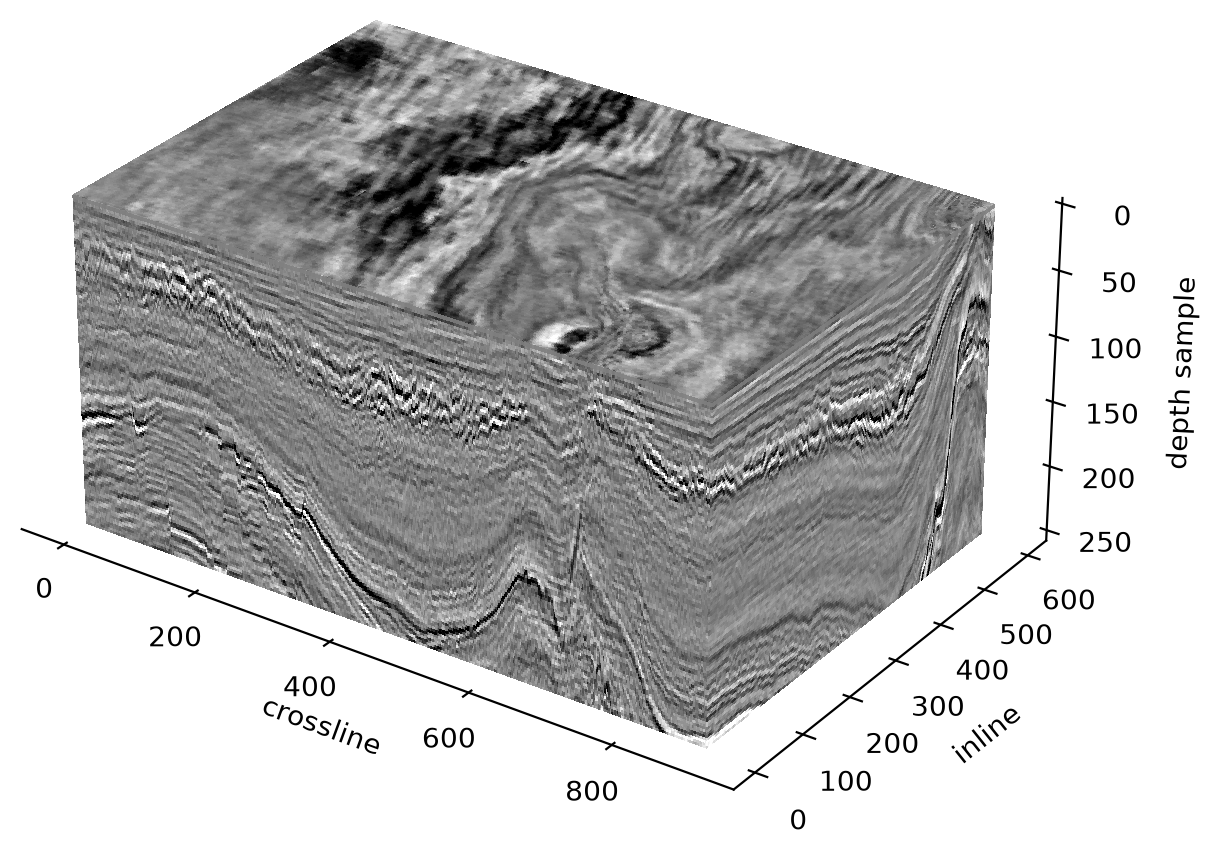
\includegraphics[width=\linewidth,height=0.70\textheight,keepaspectratio]{./solutions/fig0_seismic_cube_3d.png}
  \vspace{0.3em}
  \begin{itemize}
    \item $601$ inlines $\times$ $901$ crosslines $\times$ $253$ depth samples, shown as three orthogonal views of one volume.
    \item \textbf{Top} = depth slice (map view), \textbf{front} = inline section, \textbf{side} = crossline section.
  \end{itemize}
\end{frame}

\begin{frame}{Motivation \& experimental setup}
  \begin{itemize}
    \item \textbf{Dataset:} Full Netherlands F3 seismic cube ($601 \times 901 \times 253$ after boundary trimming).
    \item \textbf{Two evaluation settings:}
      \begin{enumerate}
        \item \textbf{2D depth-log compression:} Compress 253-sample vertical logs per trace into compact spatial embeddings ($d \in \{2, 3, 4, 8, 16, 32\}$).
        \item \textbf{3D volume reduction:} Compress 3D seismic attributes into volumetric embeddings for stratigraphy and facies analysis.
      \end{enumerate}
    \item \textbf{Baselines:} \texttt{PCA} (linear) and \texttt{UMAP} (transductive/non-parametric).
    \item \textbf{Key questions:} Does a continuous graph-kernel operator (\texttt{NOFE}) avoid seam artefacts, out-of-sample speckle and density shift? Which latent dimension and graph design best separate seismic facies?
  \end{itemize}
\end{frame}

\begin{frame}{Multi-axis stress-test overview}
  \centering
  \includegraphics[width=\linewidth,height=0.66\textheight,keepaspectratio]{./solutions/figA_nofe_radar_overview.png}
  \vspace{0.4em}
  \begin{itemize}
    \item \texttt{NOFE-8D} preserves local geometry and eliminates tile-stitching failure ($0.10$ vs.\ $1.33$ for \texttt{PCA-8D} and $1.49$ for \texttt{UMAP-8D}).
    \item Maintains Pearson $r \ge 0.990$ across $9\times$--$36\times$ sampling-density shifts.
  \end{itemize}
\end{frame}

\begin{frame}{2D depth-log compression ($253 \to 8$ dimensions)}
  \centering
  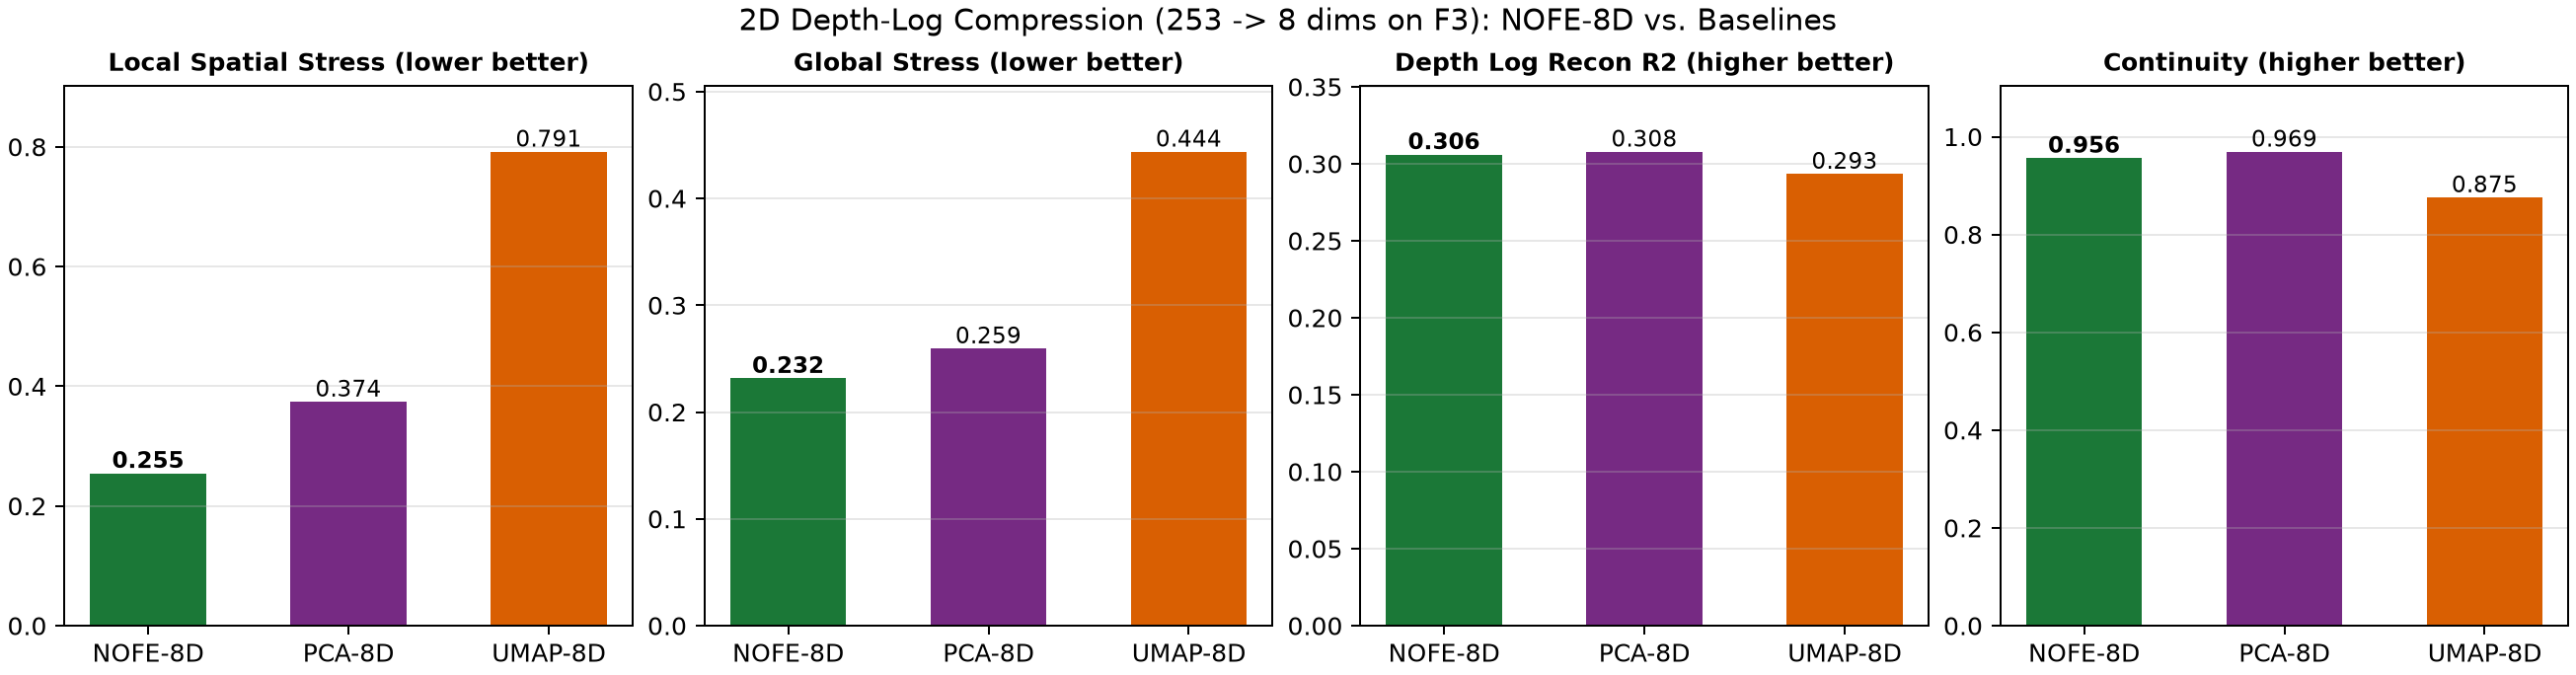
\includegraphics[width=\linewidth,height=0.58\textheight,keepaspectratio]{./solutions/fig1_depth_compression_8d_bars.png}
  \vspace{0.5em}
  \begin{itemize}
    \item Lowest \textbf{local spatial stress} ($0.258$ vs.\ $0.374$ PCA and $0.791$ UMAP) and \textbf{global stress} ($0.236$).
    \item Highest nonlinear depth-log reconstruction $R^2$ ($0.339$) with high neighbourhood continuity ($0.953$).
  \end{itemize}
\end{frame}

\begin{frame}{Four-quadrant survey stitching (visual proof)}
  \centering
  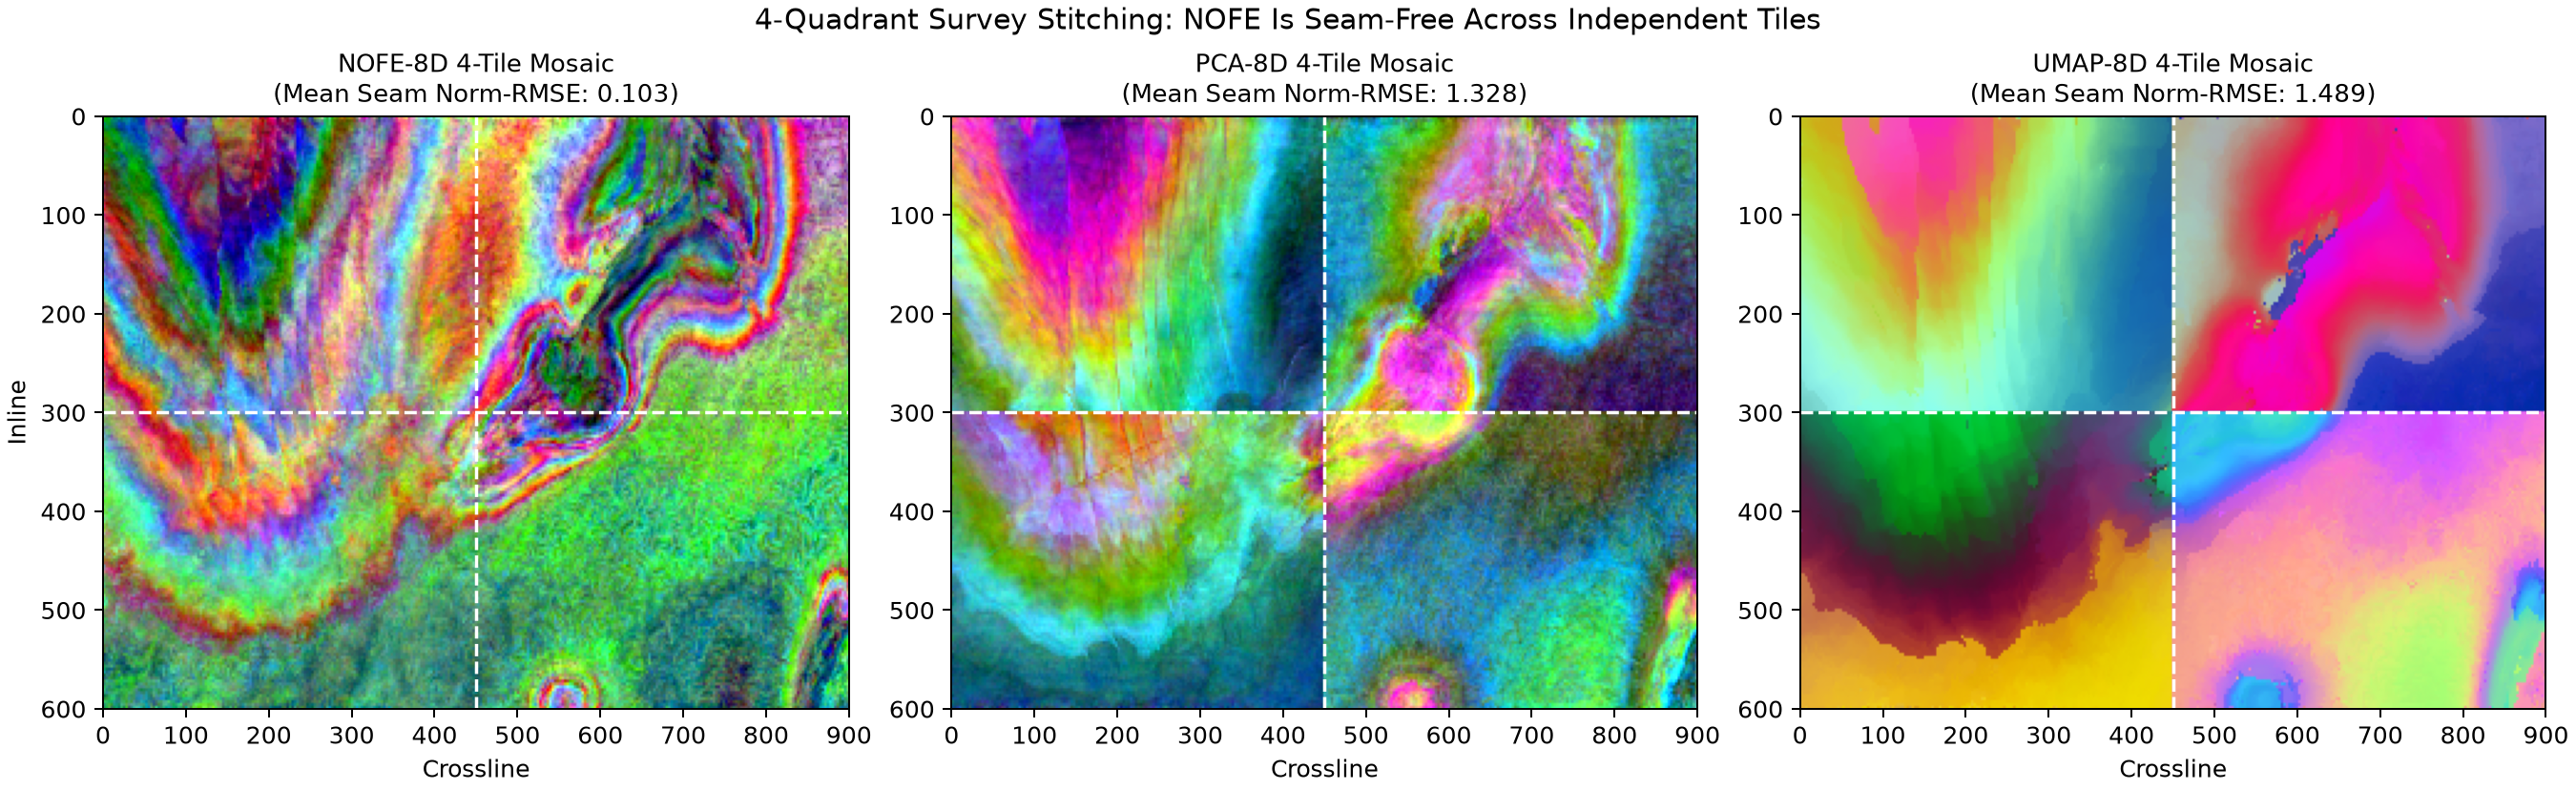
\includegraphics[width=\linewidth,height=0.60\textheight,keepaspectratio]{./solutions/figB_4tile_mosaic_seams.png}
  \vspace{0.5em}
  \begin{itemize}
    \item Four independently processed quadrants joined along dashed boundaries.
    \item \texttt{NOFE-8D} is visually seamless across tile borders (mean seam norm-RMSE $0.103$ vs.\ $1.328$ for \texttt{PCA-8D} and $1.489$ for \texttt{UMAP-8D}).
  \end{itemize}
\end{frame}

\begin{frame}{Noise robustness \& multi-density stress curve}
  \centering
  \includegraphics[width=\linewidth,height=0.68\textheight,keepaspectratio]{./solutions/figC_noise_and_density_stress.png}
  \vspace{0.3em}
  \begin{itemize}
    \item Clean-target local stress stays stable under trace noise ($\sigma \in [0, 1.0]$); zero-shot transfer tracks native $1\times 1$ from $6\times 6$ upwards.
  \end{itemize}
\end{frame}

\begin{frame}{Latent-dimension ablations ($d = 2$ to $32$)}
  \centering
  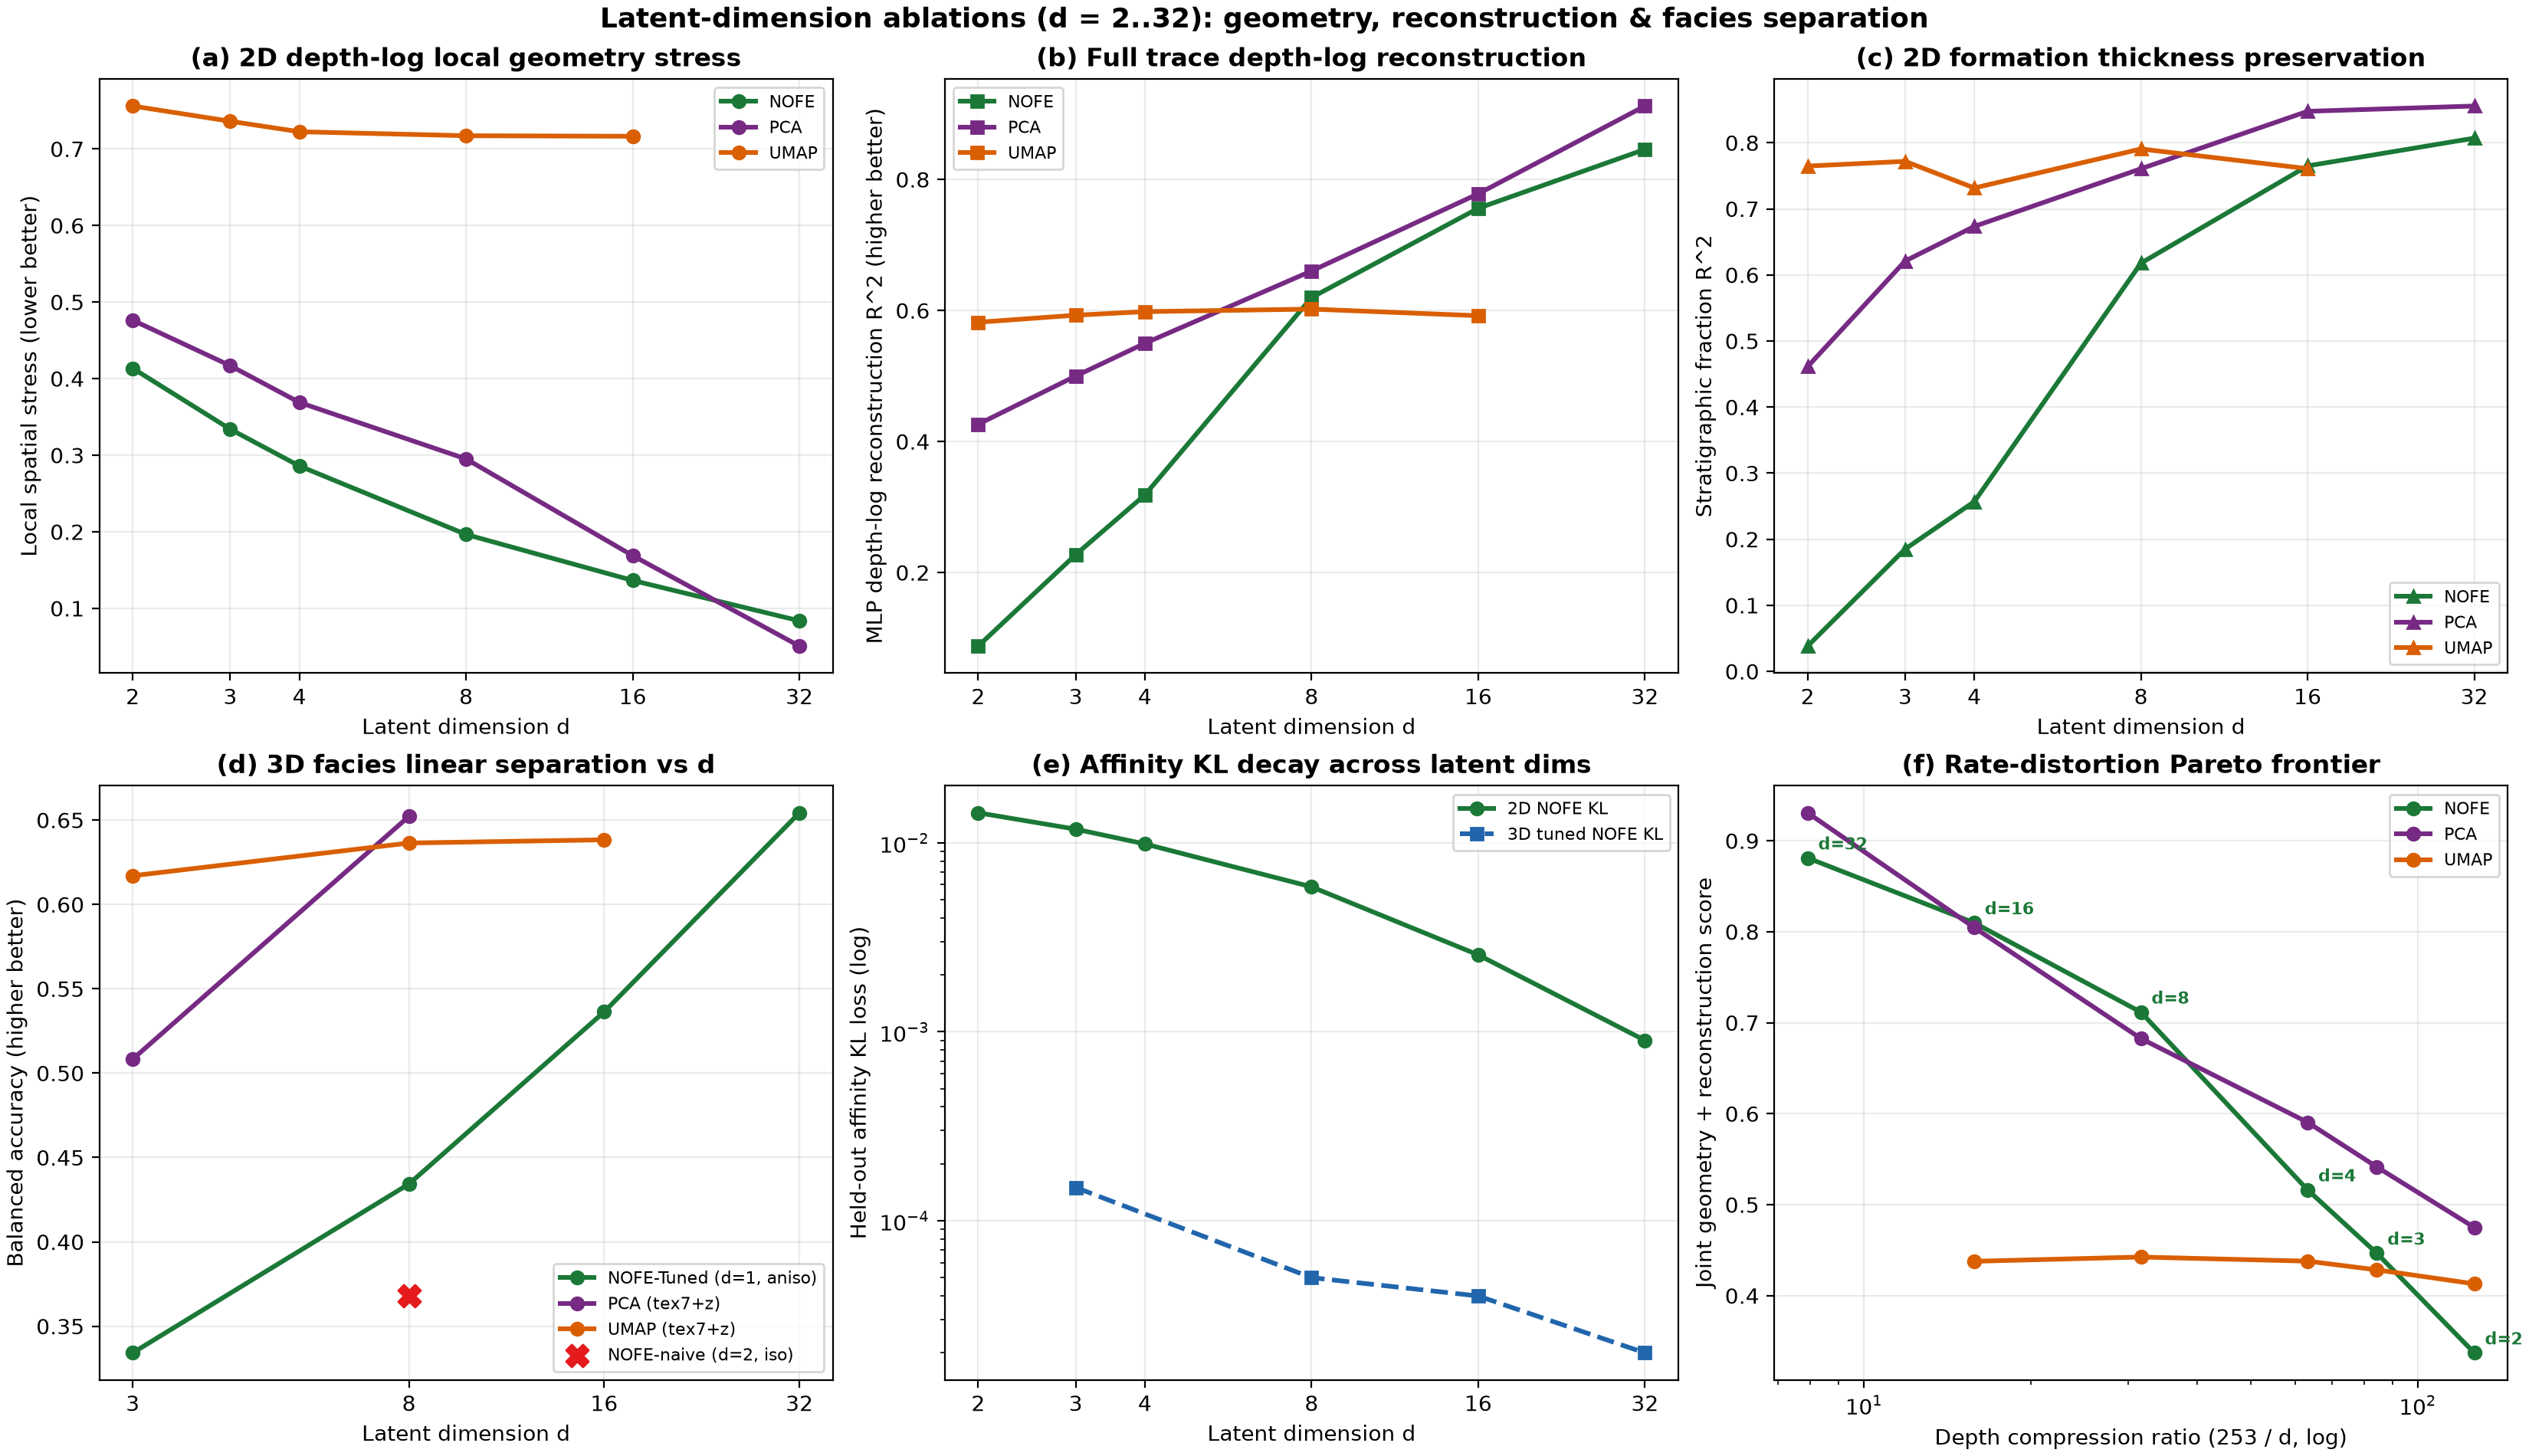
\includegraphics[width=\linewidth,height=0.62\textheight,keepaspectratio]{./solutions/ablation_latent_dim.png}
  \vspace{0.3em}
  \begin{itemize}
    \item \texttt{NOFE} achieves the lowest local spatial stress across $d = 2$--$16$ ($0.197$ at 8D and $0.136$ at 16D vs.\ $0.717$ for \texttt{UMAP}).
    \item Pareto elbows at \textbf{8D} ($31.6\times$ compression, $88.9\%$ 7-NN facies accuracy) and \textbf{16D} ($15.8\times$, $94.4\%$ accuracy, $0.765$ thickness $R^2$).
  \end{itemize}
\end{frame}

\begin{frame}{Trace-level depth-log fidelity \& unsupervised clusters}
  \centering
  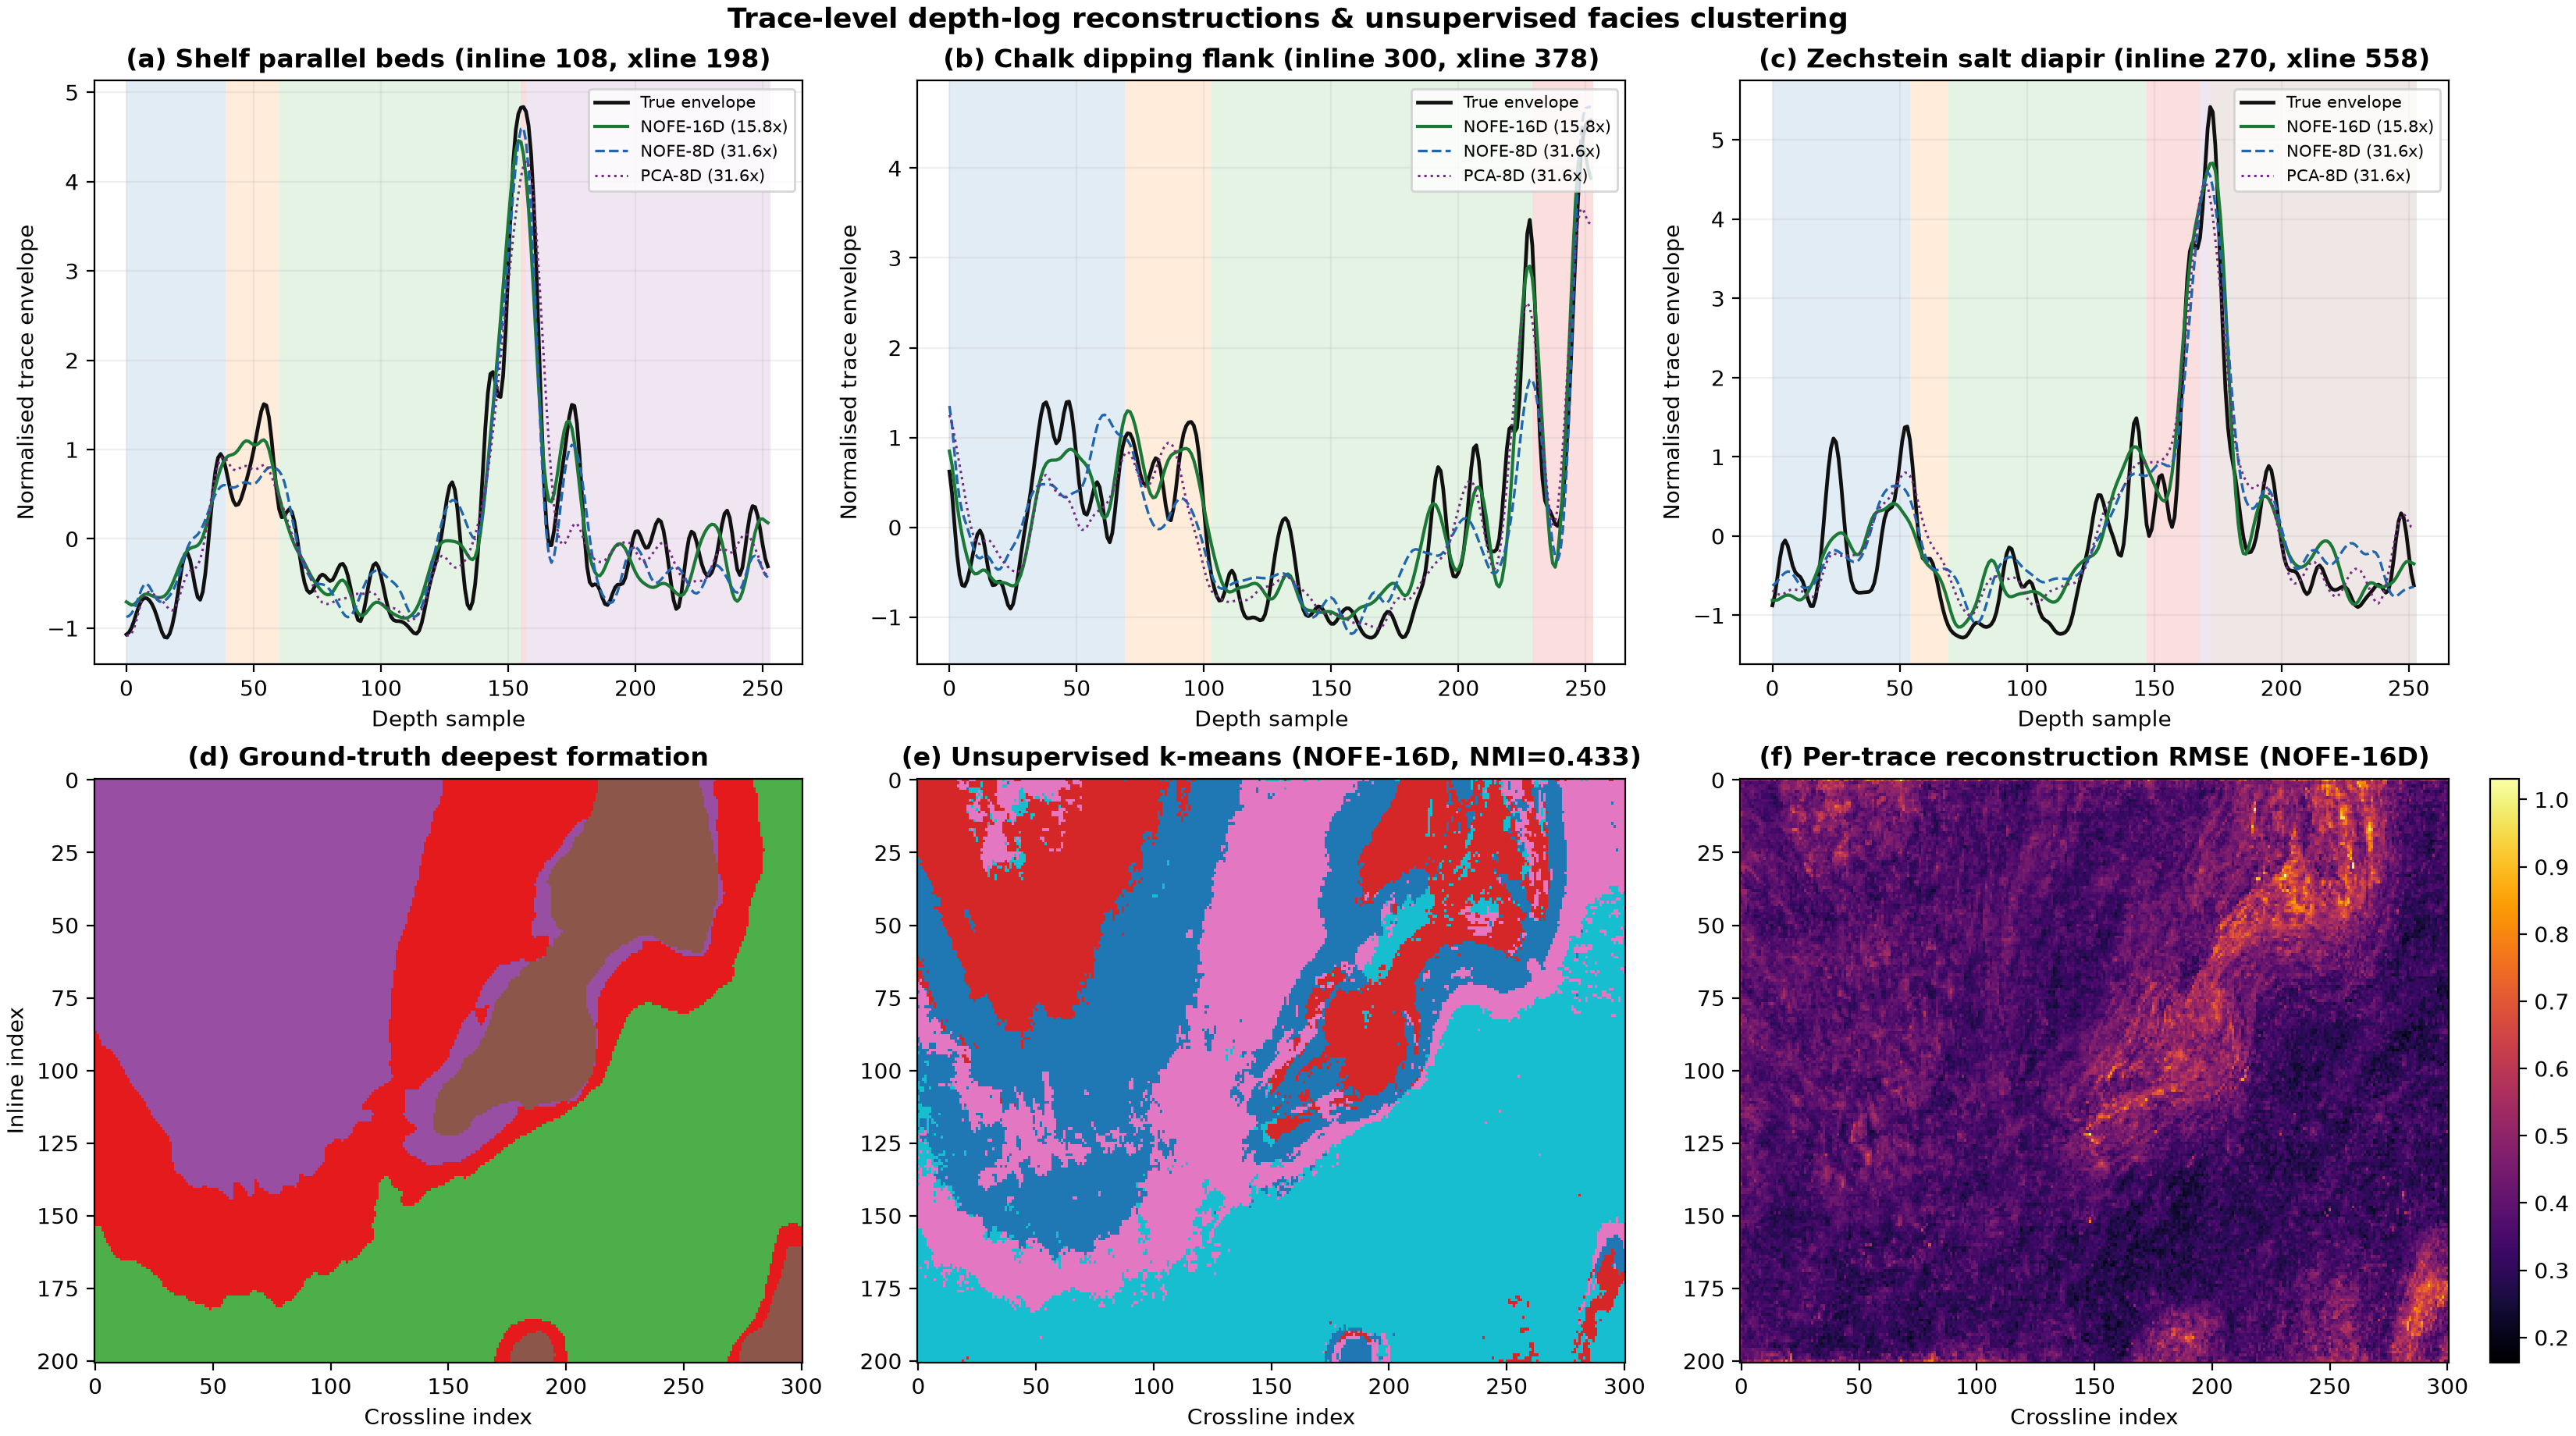
\includegraphics[width=\linewidth,height=0.62\textheight,keepaspectratio]{./solutions/trace_profiles_and_clusters.png}
  \vspace{0.3em}
  \begin{itemize}
    \item Reconstructed 2D codes track reflector peaks and unconformity transitions across shelf, Chalk flank and Zechstein diapir logs.
    \item Unsupervised $k$-means ($k=6$) on \texttt{NOFE-16D} recovers the salt diapir and basin geometry without any geological labels.
  \end{itemize}
\end{frame}

\begin{frame}{Multi-scale 2D maps \& 3D cross-section alignment}
  \centering
  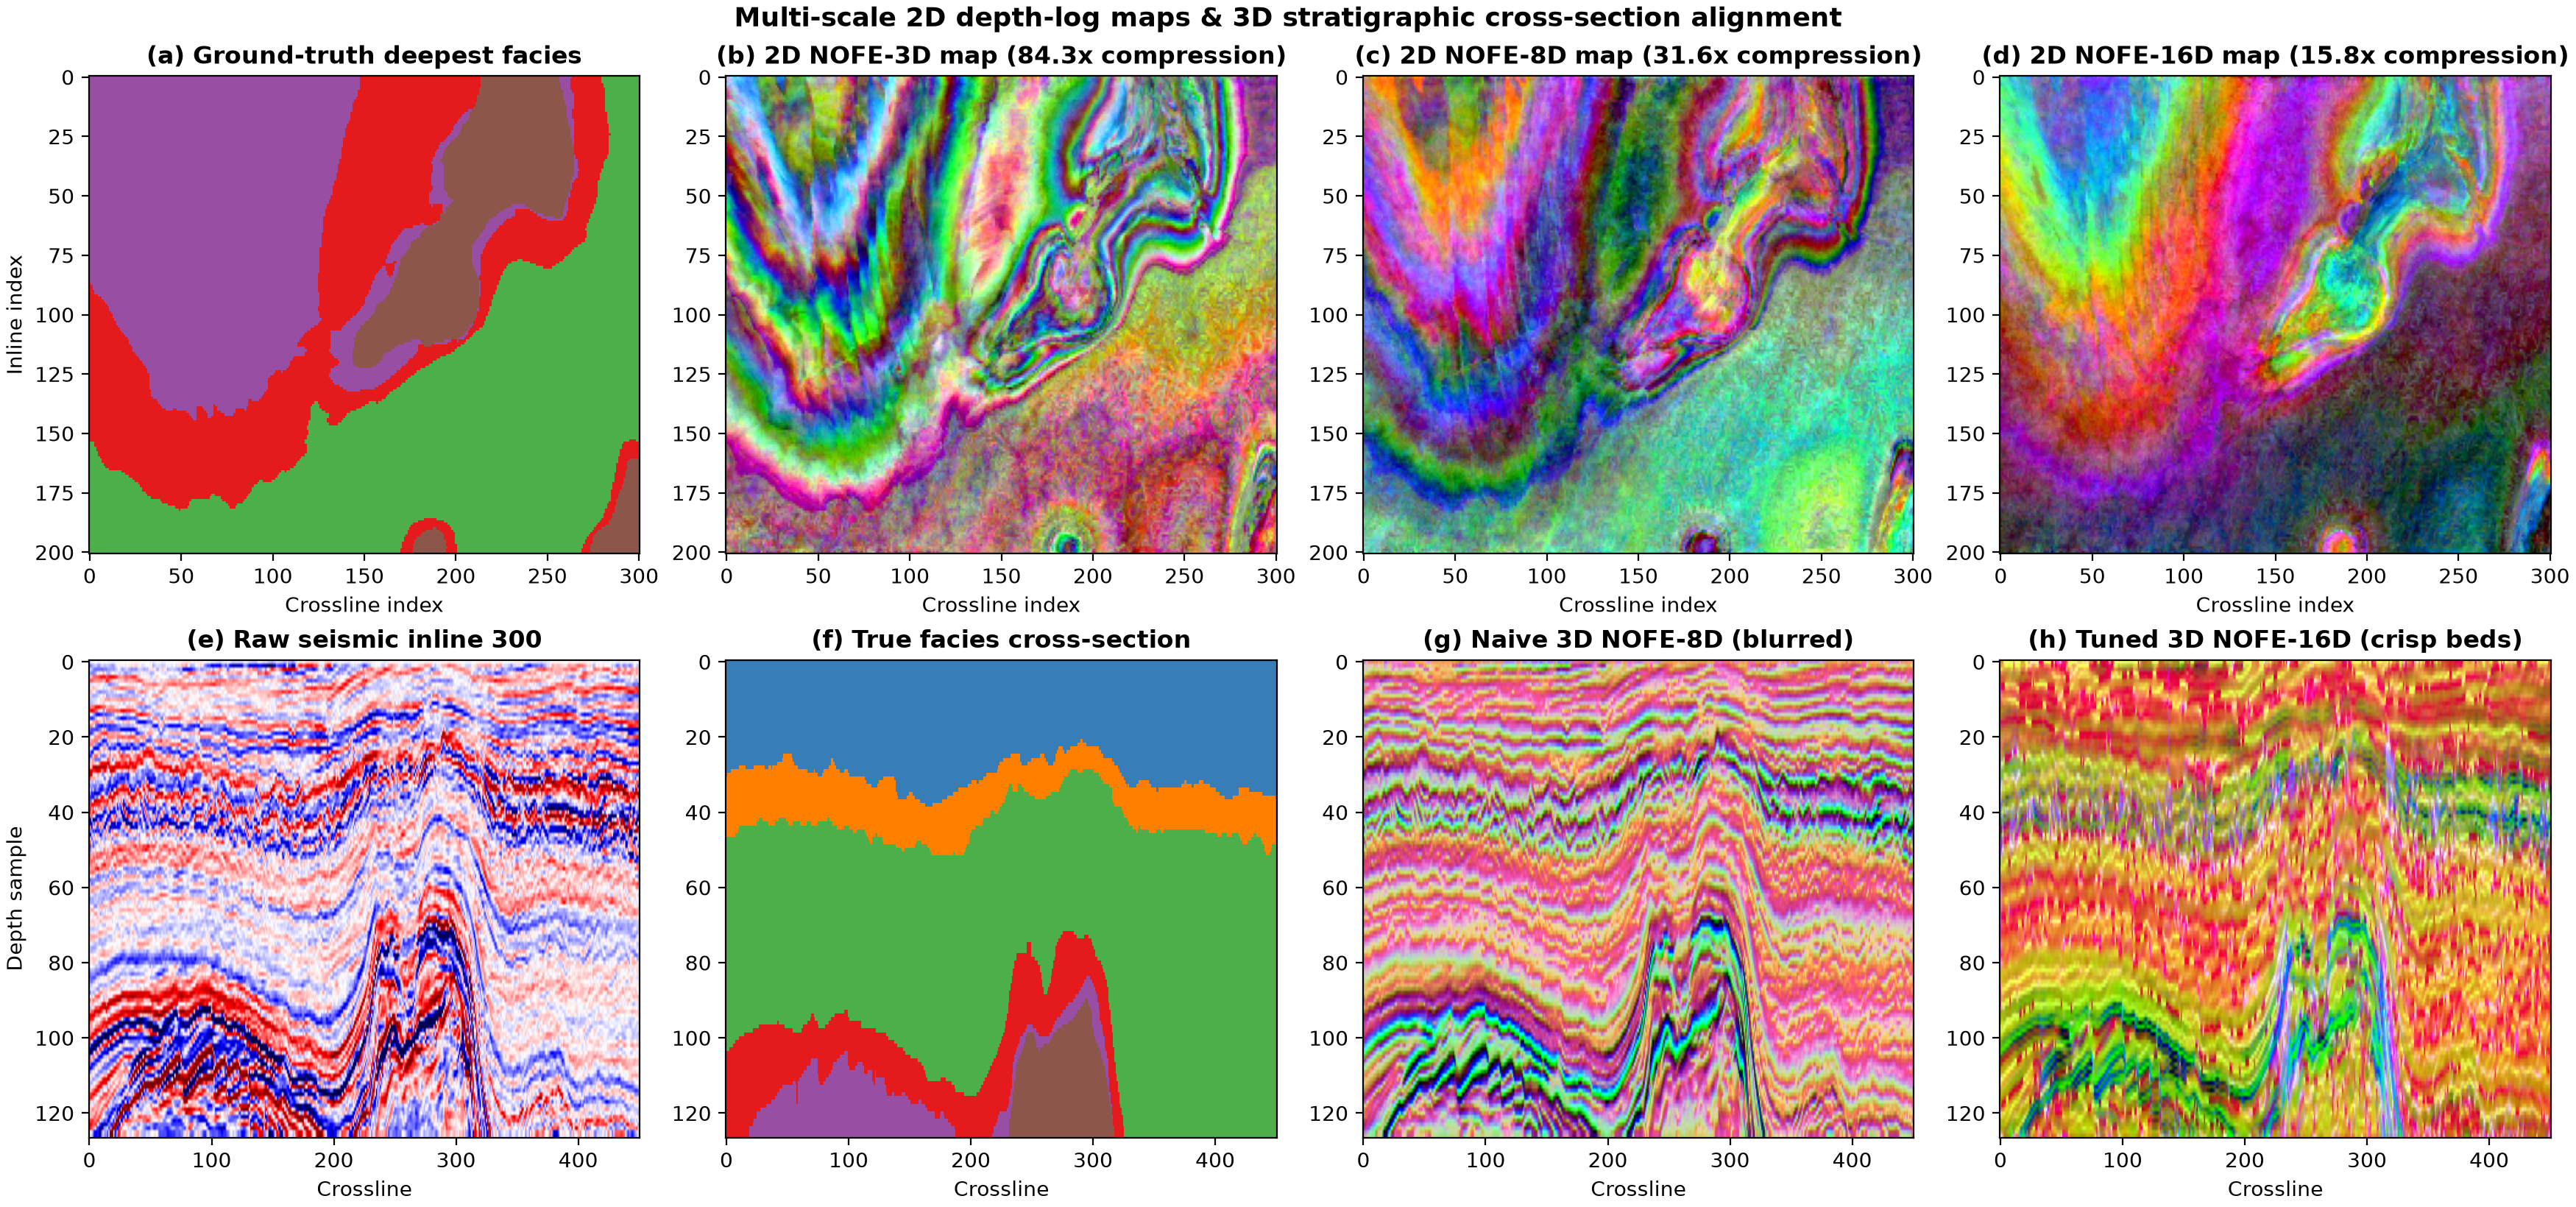
\includegraphics[width=\linewidth,height=0.62\textheight,keepaspectratio]{./solutions/multiscale_maps_cross_section.png}
  \vspace{0.3em}
  \begin{itemize}
    \item Increasing latent dimension from $3$D ($84.3\times$) to $16$D ($15.8\times$) sharpens fault and diapir boundaries on the $601 \times 901$ map.
    \item On \texttt{Inline 300}, 1-hop anisotropic 3D \texttt{NOFE-16D} replaces high-frequency phase striping with coherent stratigraphic beds.
  \end{itemize}
\end{frame}

\begin{frame}{Improving 3D facies separation}
  \centering
  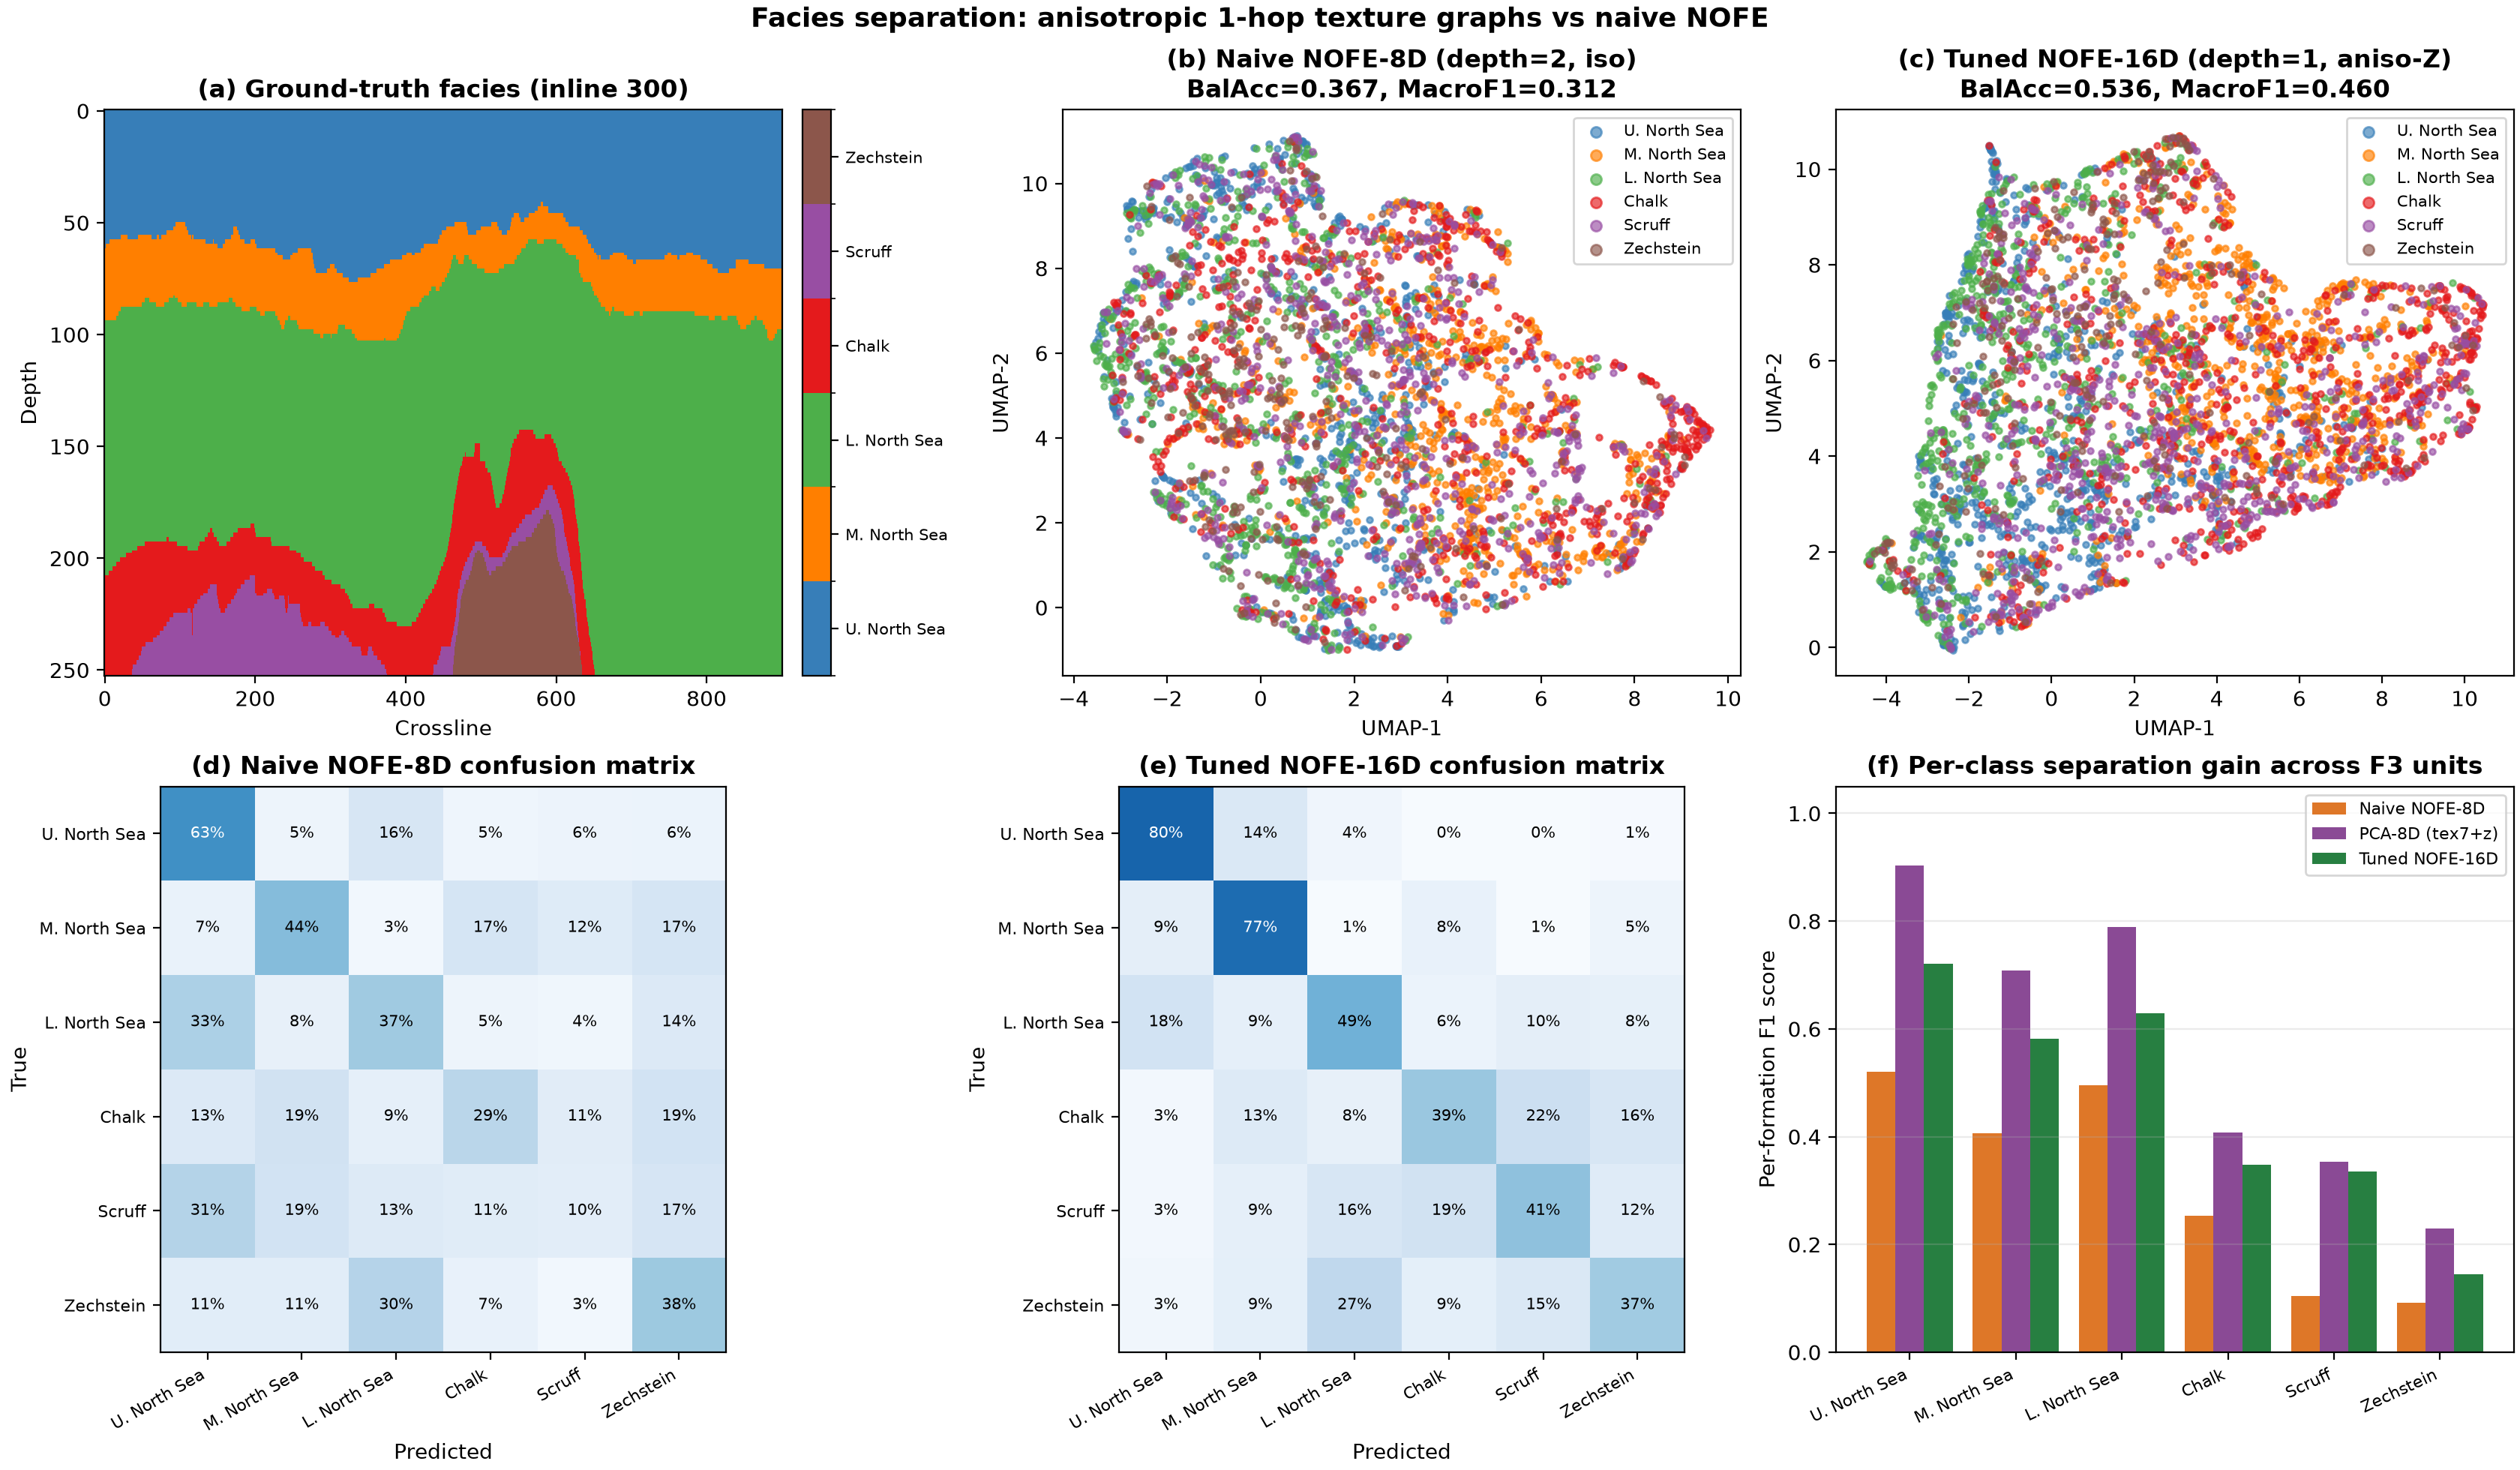
\includegraphics[width=\linewidth,height=0.60\textheight,keepaspectratio]{./solutions/facies_separation_breakthrough.png}
  \vspace{0.3em}
  \begin{itemize}
    \item \textbf{Three fixes:} 1-hop operator (\texttt{depth=1}), vertical anisotropy (\texttt{pos\_weights=(1,1,2)}) and phase-invariant texture + depth (\texttt{tex7+z}).
    \item Lifts balanced accuracy from $0.368$ (naive \texttt{NOFE-8D}) to $0.536$ (\texttt{16D}) and $0.654$ (\texttt{32D}, macro-F1 $0.559$, Scruff recall $10\% \to 41\%$).
  \end{itemize}
\end{frame}

\begin{frame}{Facies-aware 3D cutaway \& latent manifold}
  \centering
  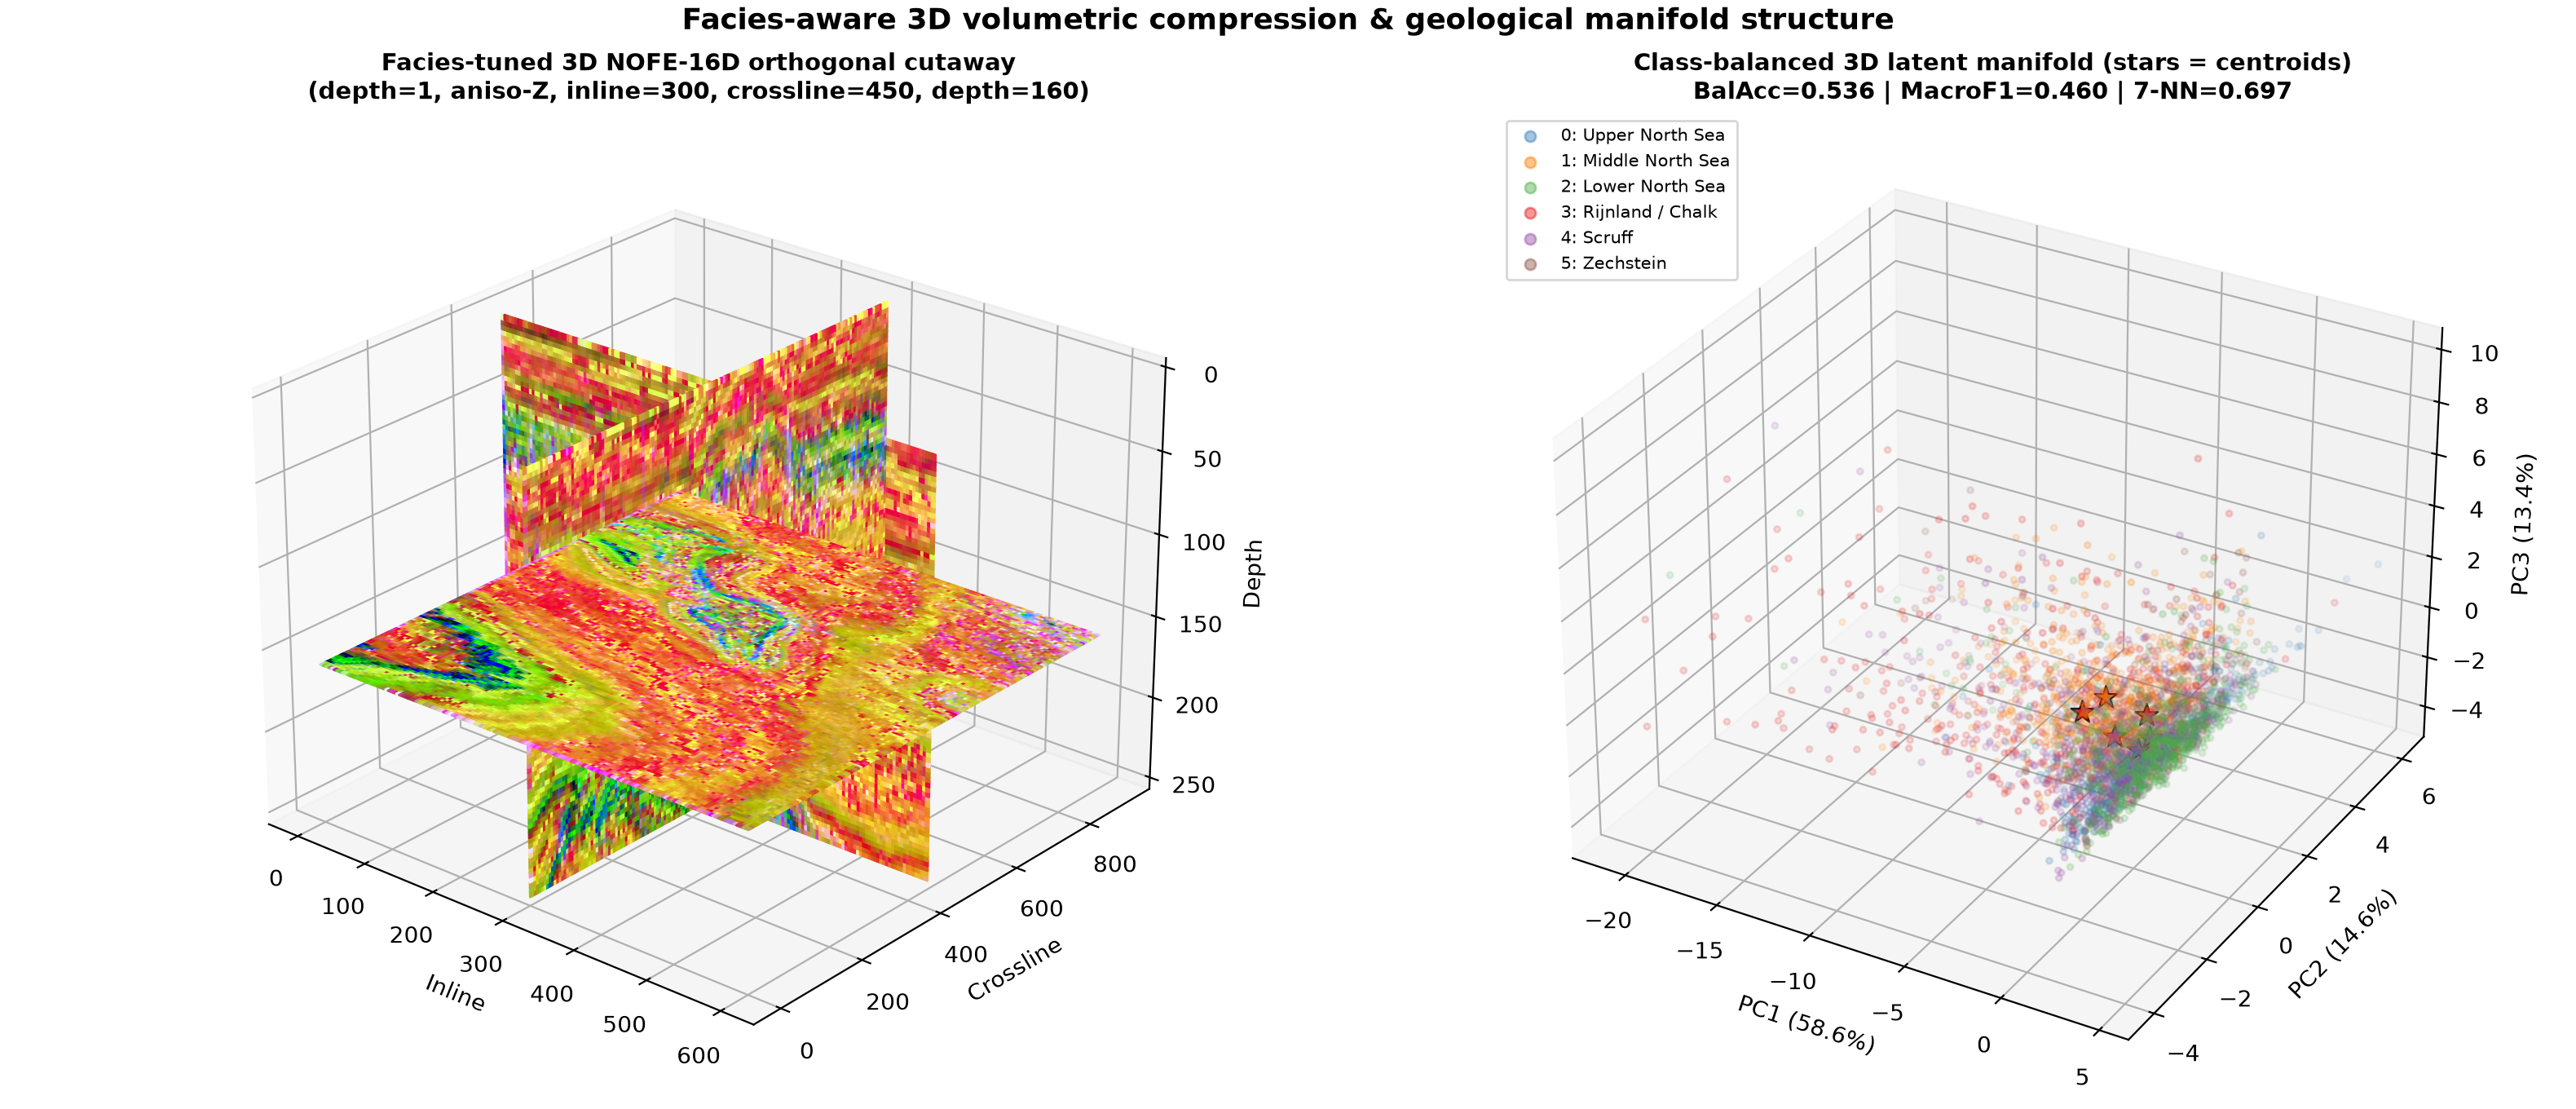
\includegraphics[width=\linewidth,height=0.65\textheight,keepaspectratio]{./solutions/hero_3d_cutaway_facies.png}
  \vspace{0.3em}
  \begin{itemize}
    \item Tuned 3D \texttt{NOFE-16D} achieves $0.041$ held-out local stress ($0.025$ at 32D vs.\ $0.427$ for \texttt{UMAP}) with clear stratigraphic ordering across orthogonal slices.
  \end{itemize}
\end{frame}

\begin{frame}{Zero-shot native-resolution salt-diapir zoom}
  \centering
  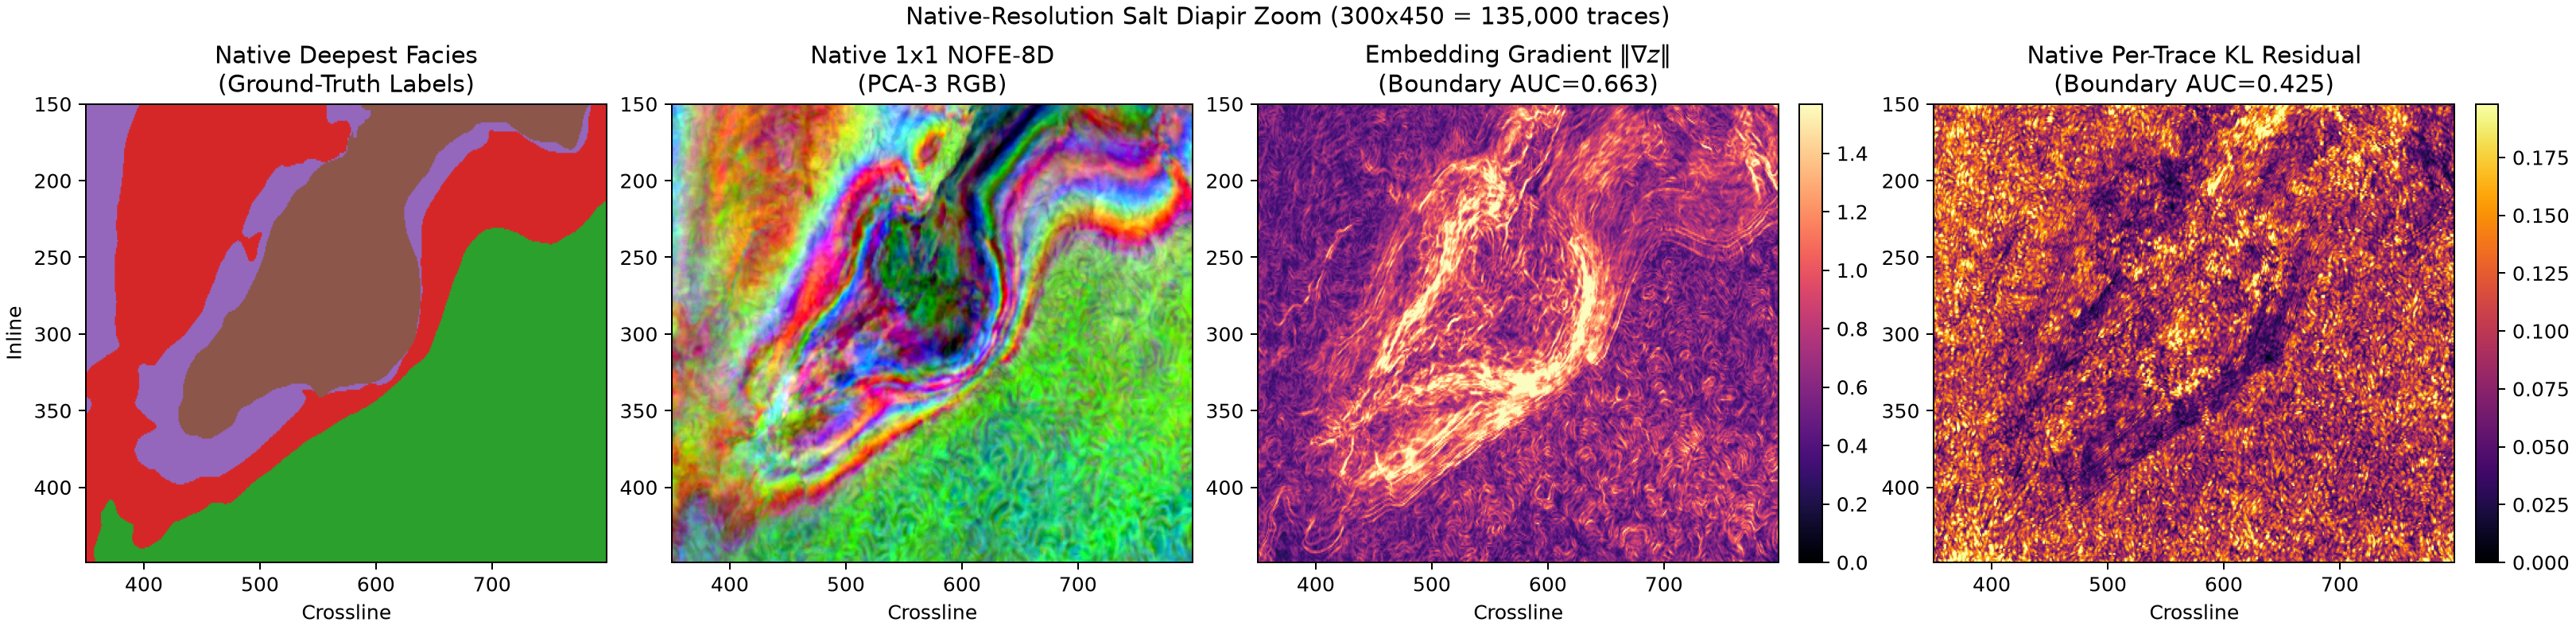
\includegraphics[width=\linewidth,height=0.58\textheight,keepaspectratio]{./solutions/figE_salt_dome_native_zoom.png}
  \vspace{0.5em}
  \begin{itemize}
    \item $300 \times 450 = 135{,}000$ traces evaluated zero-shot at native $1\times 1$ spacing.
    \item Embedding gradient $\|\nabla z\|$ sharpens salt-diapir flanks and facies boundaries (boundary AUC $= 0.667$).
  \end{itemize}
\end{frame}

\begin{frame}{Summary \& practical takeaways}
  \begin{itemize}
    \item \textbf{Continuous operator advantage:} \texttt{NOFE} eliminates tile-stitching seams ($0.103$ vs.\ $>1.32$) and transfers zero-shot across $9\times$--$36\times$ sampling changes ($r \ge 0.990$).
    \item \textbf{Latent-dimension sweet spots:} \texttt{8D} ($31.6\times$) suffices for compact mapping; \texttt{16D} ($15.8\times$) unlocks high trace reconstruction ($R^2 = 0.756$) and $94.4\%$ facies accuracy.
    \item \textbf{Facies separation recipe:} Avoiding 2-hop boundary smoothing (\texttt{depth=1}) with anisotropic bedding graphs lifts 3D balanced accuracy by $+0.286$ (to $0.654$).
    \item \textbf{Trade-off:} Global linear probes require sufficient latent capacity ($16$D--$32$D) and in-domain spatial coordinates; future work can add multi-scale global anchors without breaking local edge normalisation.
  \end{itemize}
\end{frame}

\end{document}
